\documentclass[final,hyperref={pdfpagelabels=false}]{beamer}
\usepackage{grffile}
\mode<presentation>{\usetheme{HI}}
\usepackage[english]{babel}
\usepackage[latin1]{inputenc}
\usepackage{amsmath,amsthm, amssymb, latexsym}
%\usepackage{times}\usefonttheme{professionalfonts}  % obsolete
%\usefonttheme[onlymath]{serif}
\boldmath
\usepackage[orientation=portrait,size=a0,scale=1.4,debug]{beamerposter}
% change list indention level% \setdefaultleftmargin{3em}{}{}{}{}{}
\usepackage{tcolorbox}
\usepackage{color}

%\usepackage{snapshot} % will write a .dep file with all dependencies, allows for easy bundling

\usepackage{array,booktabs,tabularx}
\newcolumntype{Z}{>{\centering\arraybackslash}X} % centered tabularx columns
\newcolumntype{C}[1]{>{\centering\let\newline\\\arraybackslash\hspace{0pt}}m{#1}}

\listfiles

%%%%%%%%%%%%%%%%%%%%%%%%%%%%%%%%%%%%%%%%%%%%%%%%%%%%%%%%%%%%%%%%%%%%%%%%%%%%%%%%%%%%%%
\graphicspath{{figures/}}
 
\title{\huge Exploring uncertainties and subjective decisions in ecosystem modeling: the Icelandic Atlantis model}
\author{Christopher David Desjardins, Bjarki Elvarsson, Erla Sturludottir, \& Gunnar Stefansson}
\institute[RWTH Aachen University]{Science Institute - University of Iceland, Reykjavik, Iceland}
\date[Sep. 8th, 2009]{Sep. 8th, 2009}

%%%%%%%%%%%%%%%%%%%%%%%%%%%%%%%%%%%%%%%%%%%%%%%%%%%%%%%%%%%%%%%%%%%%%%%%%%%%%%%%%%%%%%
\newlength{\columnheight}
\setlength{\columnheight}{100cm}


%%%%%%%%%%%%%%%%%%%%%%%%%%%%%%%%%%%%%%%%%%%%%%%%%%%%%%%%%%%%%%%%%%%%%%%%%%%%%%%%%%%%%%
\begin{document}
\begin{frame}
\vspace{.8cm}
  \begin{columns}
    % ---------------------------------------------------------%
    % Set up a column 
    \begin{column}{1\textwidth}
      \begin{beamercolorbox}[center,wd=\textwidth]{postercolumn}
        \begin{minipage}[T]{.98\textwidth}  % tweaks the width, makes a new \textwidth
          \parbox[t][\columnheight]{\textwidth}{ % must be some better way to set the the height, width and textwidth simultaneously
            % Since all columns are the same length, it is all nice and tidy.  You have to get the height empirically
            % ---------------------------------------------------------%
            % fill each column with content    
            \setbeamertemplate{block begin}[notitle]        
            \begin{block}{}
            \begin{columns}
            \begin{column}{.49\textwidth}
              
              \centering \textbf{Introduction}
              \begin{itemize}
              \item Atlantis is a whole-of-system ecosystem model
              \item Deterministic biodemographic and biogeochemical box model
              \item Tracks the flow of nitrogen through biological and detrital groups
              \item Includes the following submodels:
                \begin{itemize}
                \item Oceanographic
                \item Biological
                \item Fisheries
                \item Economic
                \item Assessment
                \end{itemize}
              \item Models all the major processes
              \item Models invertebrates as biomass pools (mg N/m$^2$ or mg N/m$^3$) and vertebrates as age-structured models
              \item Intended to be used strategically not tactically
              \item Data intensive
              \item \underline{Uncertainty and subjectivity during model development and calibration}
              \end{itemize}
              \end{column}
               \begin{column}{.49\textwidth}
              \centering \textbf{Modelling decisions}
              \begin{itemize}
              \item Spatial structure
              \item Diet/prey availability
              \item Functional group assemblages
              \item Consumption \& growth
              \item Mortality
              \item \underline{Tuning is model specific, can not start with simple model}
               \end{itemize}
               
               \vspace{.5cm}
               \centering \textbf{Iceland Atlantis Model}
               \vspace{1cm}
               
               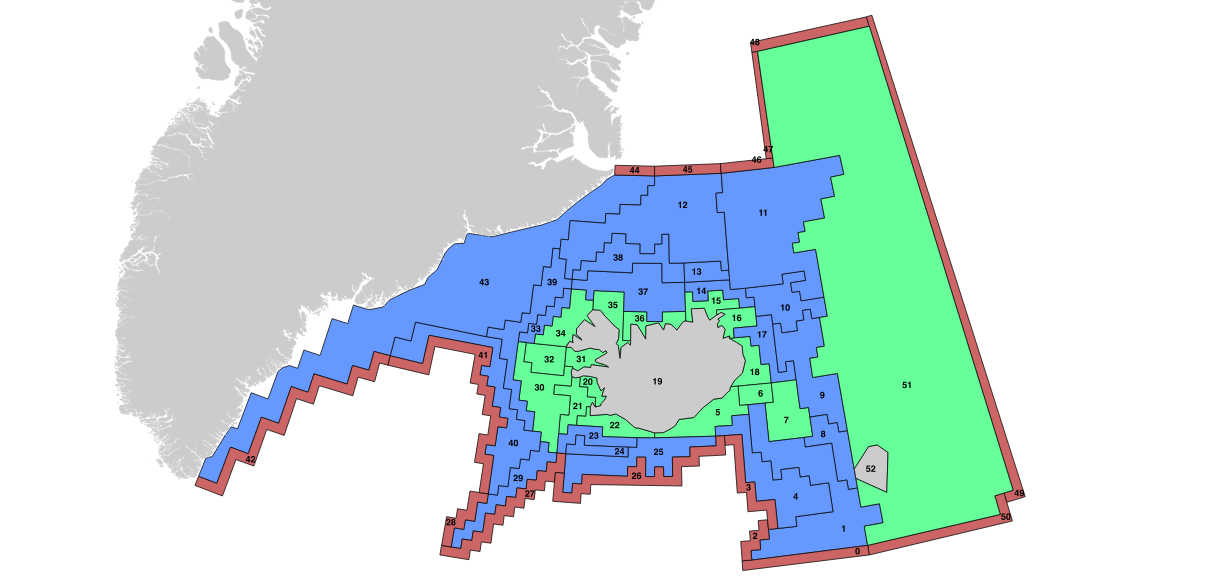
\includegraphics[scale = .5]{images/atlantis_with_layers_colored.png}
               \end{column}
              \end{columns}    
                       
            \end{block}

          
          \vspace{1cm}
            \begin{block}{}
            \begin{columns}
            \begin{column}{.85\textwidth}
            
            \centering \textbf{Prey availability}
              \begin{figure}
              \centering
              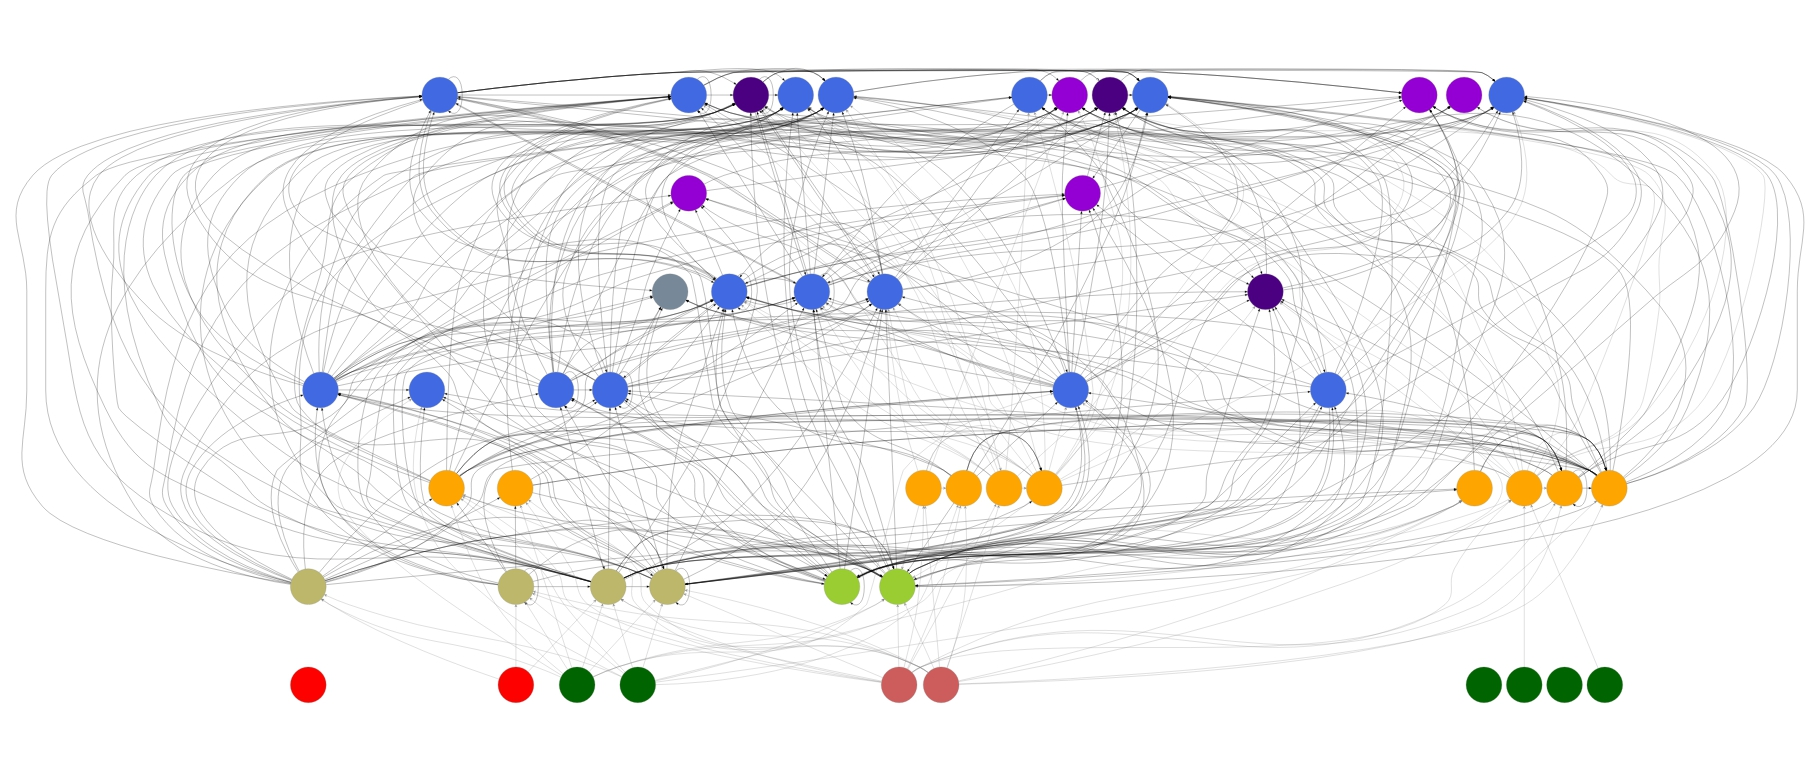
\includegraphics[height = 30cm]{images/food_web.jpeg}
                \footnotesize
                   \end{figure}
              \end{column}
              \begin{column}{.15\textwidth}
              \begin{figure}
              \centering
              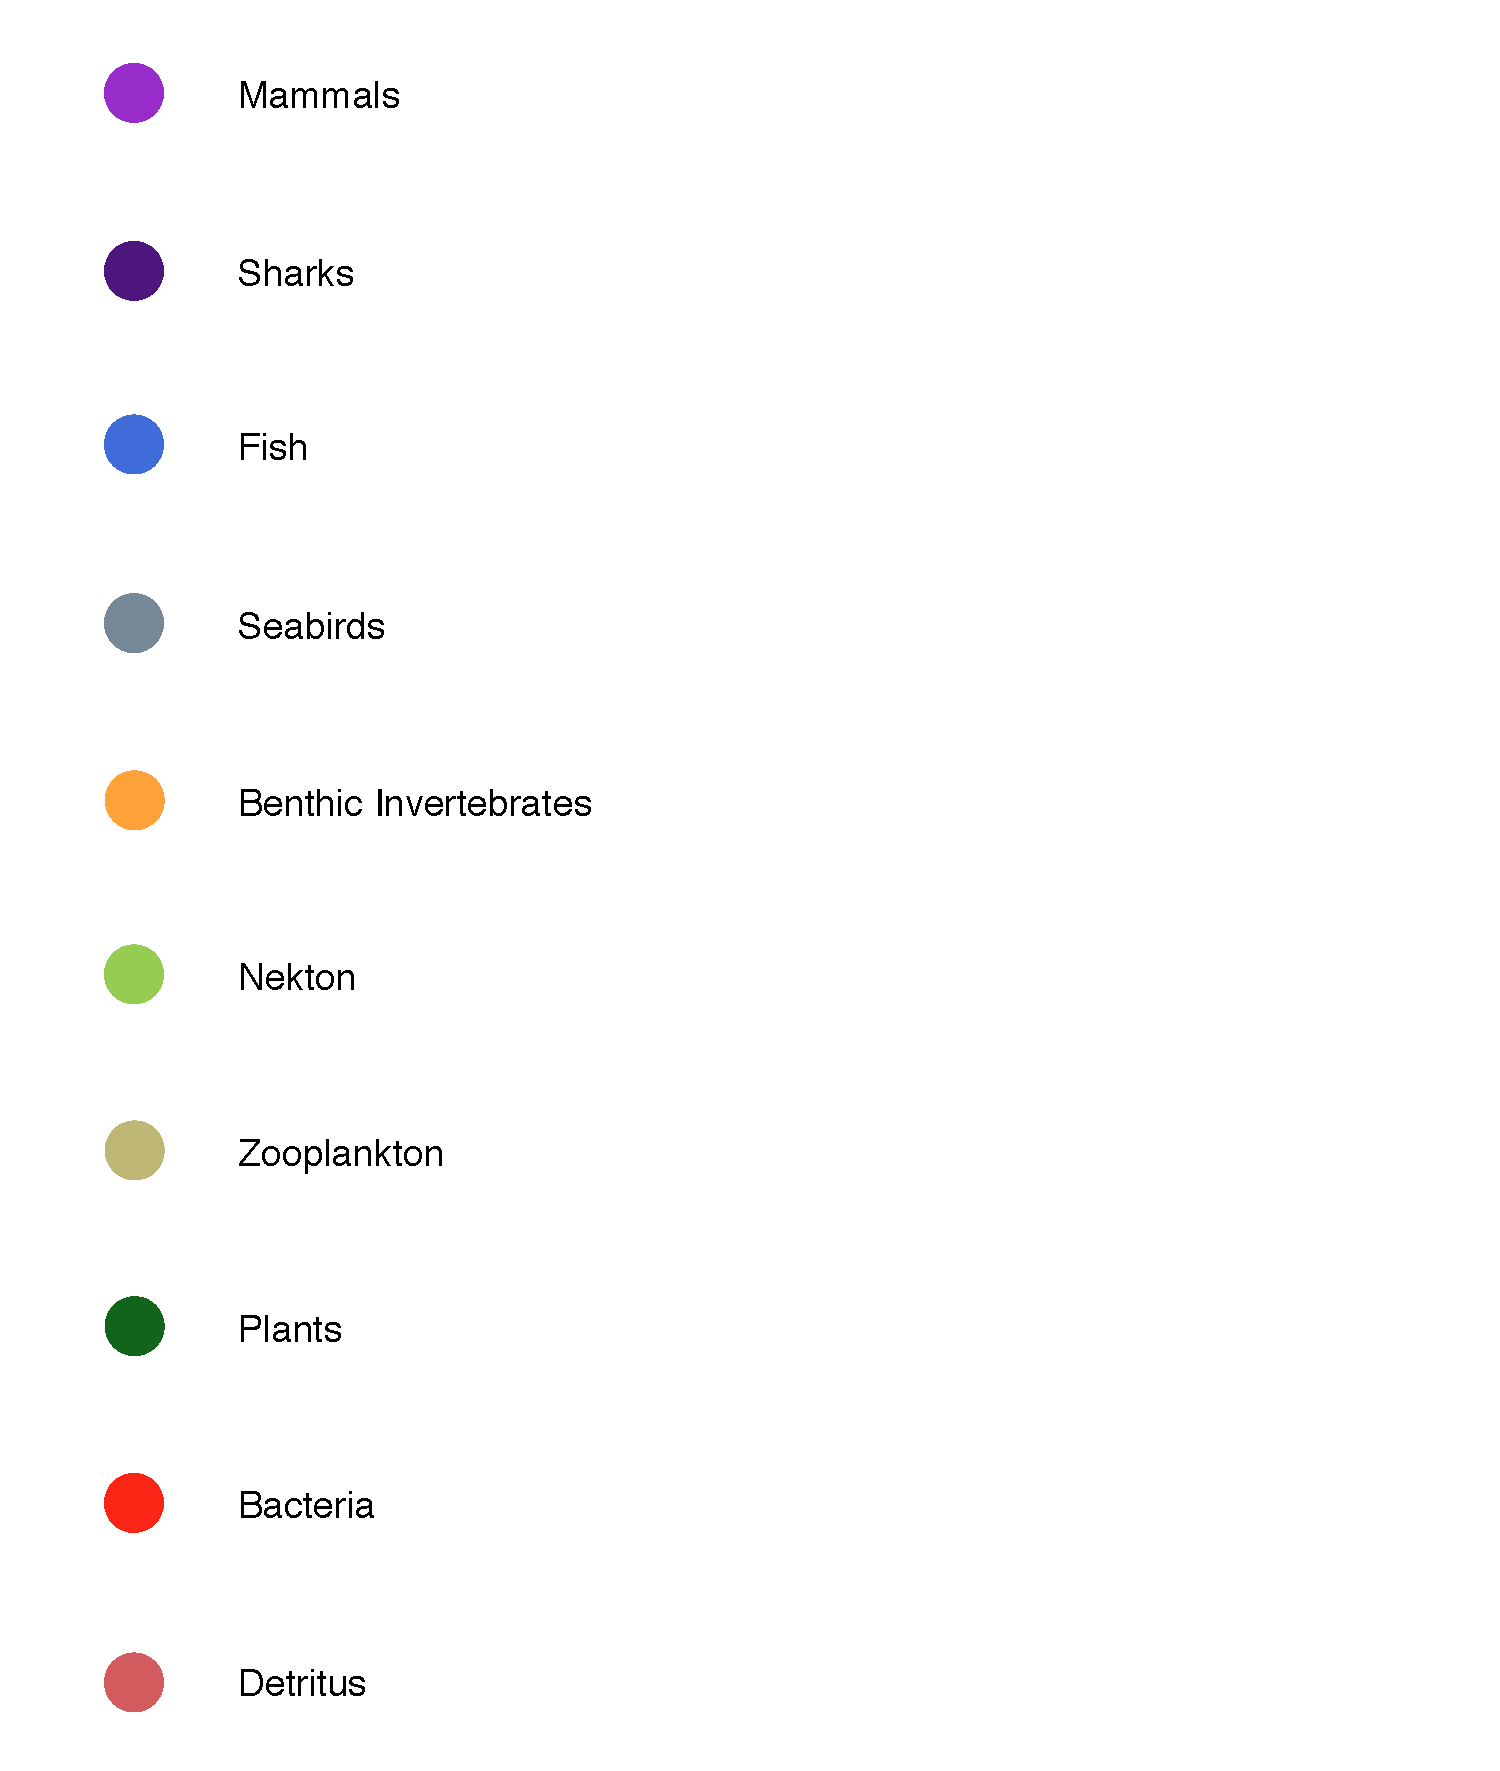
\includegraphics[height = 30cm]{images/food_web_legend.pdf}
                \footnotesize
                   \end{figure}
                   \end{column}
              \end{columns}
            \end{block}
            
            \vspace{1cm}
            \begin{block}{stuff}
            \begin{columns}
            \begin{column}{.49\textwidth}
            
            \centering \textbf{Functional group assemblages}
            
            \begin{itemize}
            	\item 52 functional groups
		\item Individual or aggregates
		\item Determined based on expert opinion or cluster analysis
            \end{itemize}
            
            \begin{center}
            \begin{tabular}{p{.5\linewidth}p{.3\linewidth}}
            \hline
            Type & Number of groups \\
            \hline
            Bony fish & 16 \\
            Cartilaginous fish & 3 \\
            Seabirds & 1 \\
            Pinnipeds & 1 \\
            Baleen whales & 2 \\
            Toothed whales & 2\\
            Shrimp & 1 \\
            Cephlapods & 1\\
            Zooplankton & 4 \\
            Benthic invertebrates & 10 \\
            Phytoplankon & 3 \\
            Plants & 3 \\
            Bacteria & 2 \\
            Detritus & 2\\
            \hline
            \end{tabular}
            \end{center}
           
              \vspace{.5cm}
               \centering \textbf{Tuning parameters}
               \vspace{.5cm}
            
            \begin{itemize}
            \item Can get initial estimates for many parameters
	  \item However, many parameters must be tuned to prevent explosion or extinction
	\item How tuning is done:
		\begin{itemize}
			\item \underline{Subjectively}: change parameters and see how it changes visually 
			\begin{itemize}
			\item \underline{Visualising Atlantis toolbox} created for this purpose
			\end{itemize}
			\item \underline{Objectively}: series of parallel runs with one parameter change, minimize some objective function, and select these parameters 
		\end{itemize}
            \end{itemize}
            \end{column}
            \begin{column}{.49\textwidth}
            
    
           
              \centering \textbf{Visualising Atlantis Toolbox}
            
            \begin{itemize}
            	\item Software created at the University of Iceland as part of the MareFrame project to aid in model tuning and calibration
	\item It is an installable R package that is run like any ordinary R function
	\item Consists of the following modules:
		\begin{itemize}
			\item Interactive spatially disaggregated plots for all functional groups and tracers
			\item Animated plots
			\item Aggregated (over time and age-class) and summary plots
			\item Diet plots and matrices
		\end{itemize}
	\item Code is open-sourced, GPL'ed, and available at: \textcolor{blue}{https://github.com/cddesja/vat}
	\item Demonstration of the program at: \textcolor{blue}{http://130.208.71.121:3838/vat/}
            \end{itemize}
            
            \vspace{1cm}
            \begin{tabularx}{\linewidth}{ZZZ}

      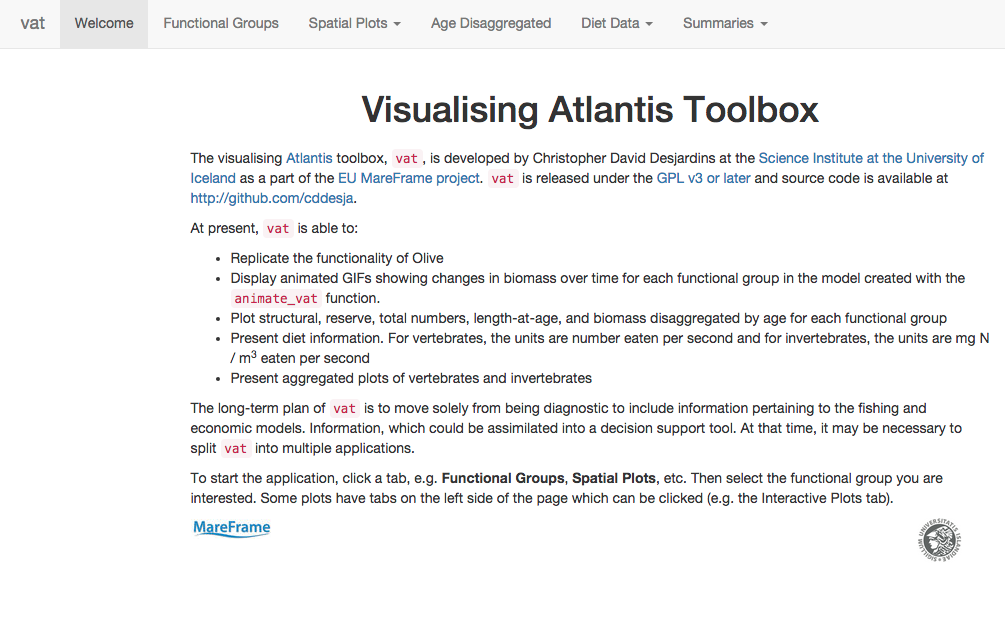
\includegraphics[width=1\linewidth]{images/vat1.png} & 
            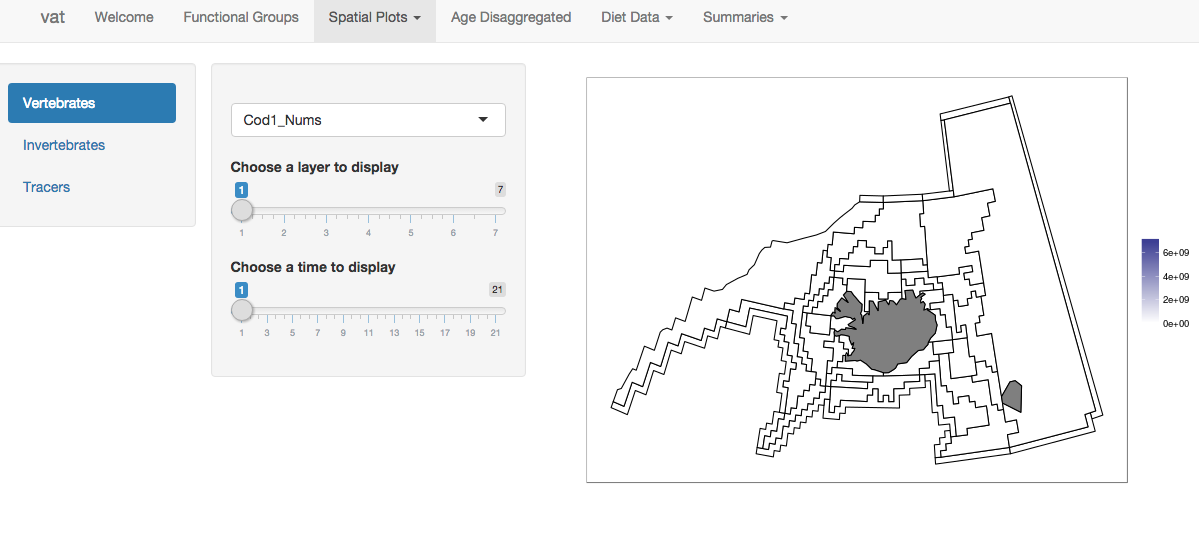
\includegraphics[width=1\linewidth]{images/vat2.png} &
                  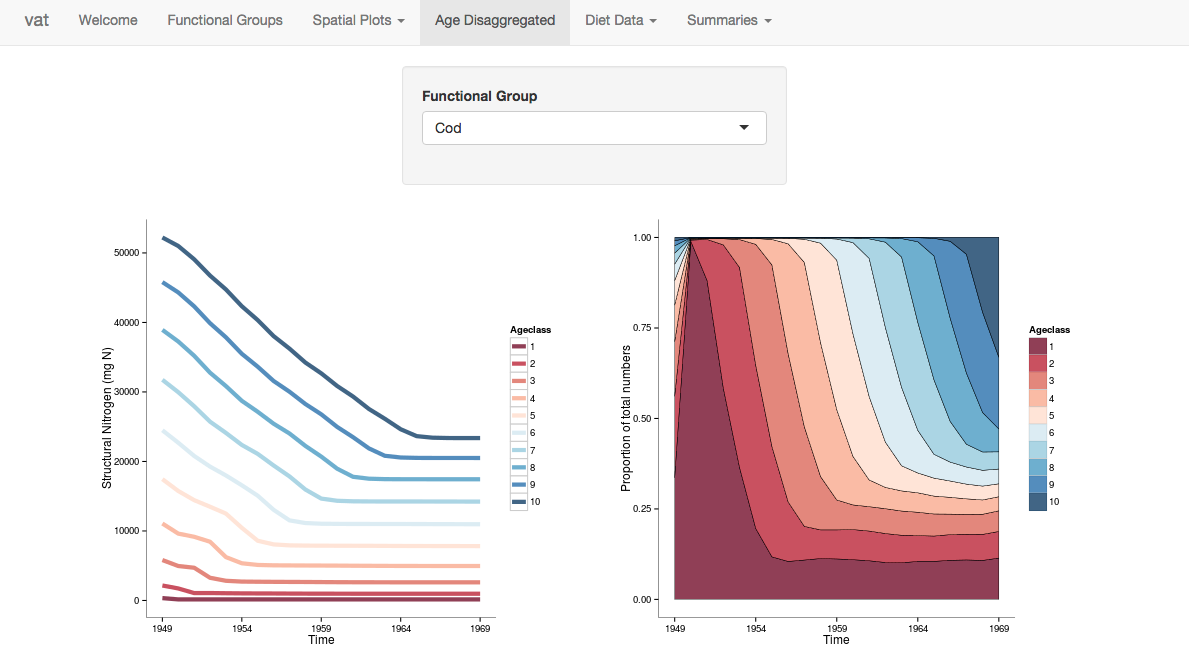
\includegraphics[width=1\linewidth]{images/vat3.png} \\
                  \\
                   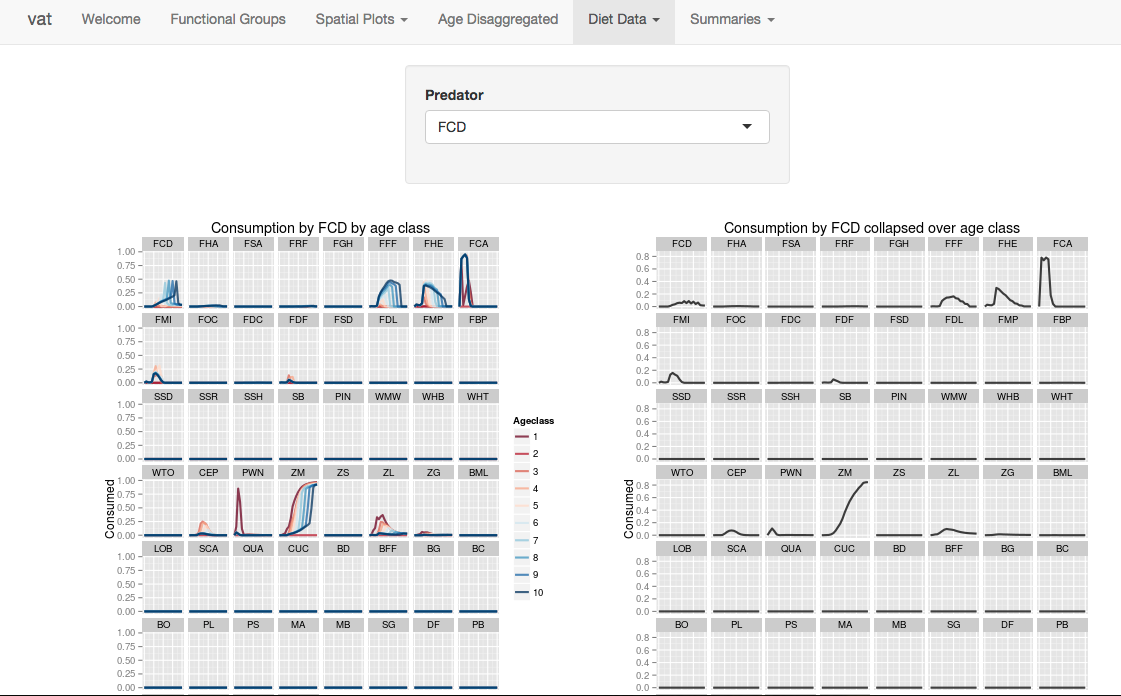
\includegraphics[width=1\linewidth]{images/vat4.png} & 
            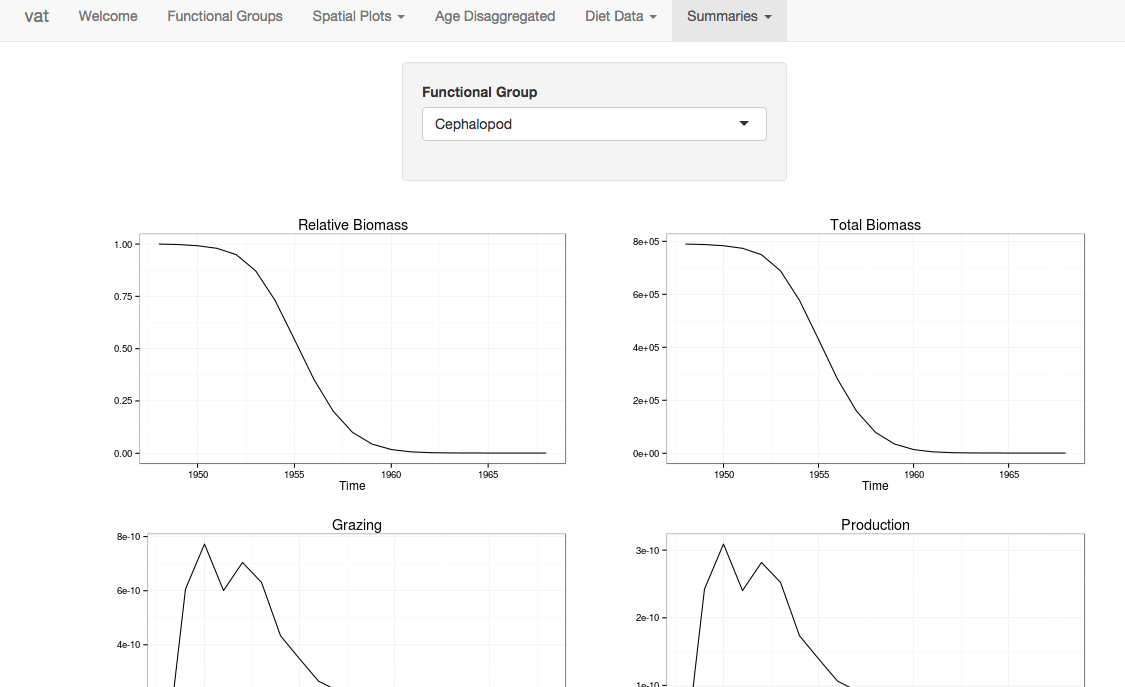
\includegraphics[width=1\linewidth]{images/vat5.png} &
                  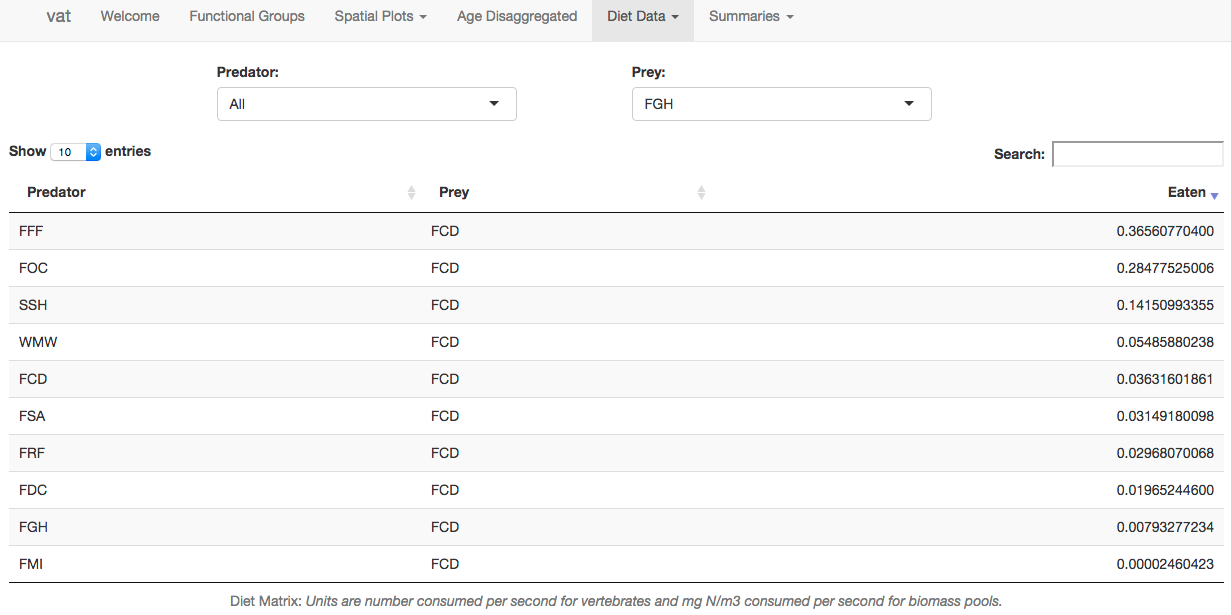
\includegraphics[width=1\linewidth]{images/vat6.png}

            
            \end{tabularx}
            \begin{flushright}
            
\includegraphics{images/mf_logo.pdf}
            \end{flushright}
            \end{column}
            
            \end{columns}
            \end{block}
            \vfill
          }
        \end{minipage}
      \end{beamercolorbox}
    \end{column}

  \end{columns}
  \vfill
  %\tiny\hfill\textcolor{ta2gray}{Created with \LaTeX \texttt{beamerposter}  \url{http://www-i6.informatik.rwth-aachen.de/~dreuw/latexbeamerposter.php}}
  \vspace{4.5cm}
  \tiny\hfill{Created with \LaTeX \texttt{beamerposter}  \url{http://www-i6.informatik.rwth-aachen.de/~dreuw/latexbeamerposter.php} \hskip1em}
\end{frame}
\end{document}


%%%%%%%%%%%%%%%%%%%%%%%%%%%%%%%%%%%%%%%%%%%%%%%%%%%%%%%%%%%%%%%%%%%%%%%%%%%%%%%%%%%%%%%%%%%%%%%%%%%%
%%% Local Variables: 
%%% mode: latex
%%% TeX-PDF-mode: t
%%% End:
